\chapter{Untersuchung von MorphNet}\label{sec:morphexperimente}

Die in Kapitel \ref{sec:morphnet} erläuterte Methode zum ``schnellen Ressourcen beschränkten Strukturlernen'' (MorphNet) wird in diesem Kapitel evaluiert. In Algorithmus \ref{alg:morphnet} wird das Vorgehen von MorphNet mittels Pseudocode dargestellt. Im ersten Schritt zur Evaluierung werden die einzelnen Schritte in diesem Algorithmus evaluiert. Im zweiten Schritt wird dann überprüft, wie gut der Algorithmus mit den in Kapitel \ref{sec:konzept} genannten Rahmenbedingungen abschneidet. Da für ide Untersuchung der einzelnen Schritte von MorphNet die Ausführungszeit unwichtig ist wird dieser Teil auf der Geforce GTX 1080 Ti ausgeführt.

\section{Evaluierung der einzelnen Schritte von MorphNet}
Im ersten Schritt von MorphNet wird das Netz trainiert um 
\begin{equation}
\mathcal{W}^{\ast}=\underset{\mathcal{W}}{arg min}\; l(f(\mathbf{x_i}, \mathcal{W},y_i) + \lambda \mathcal{G}(\mathcal{W}))
\end{equation}
zu finden. Der Regularisierer $\mathcal{G}$ ist in dieser Formel dafür zuständig, dass die gewählte Zielgröße minimiert wird. Die zwei möglichen Zielgrößen sind die Modellgröße und Anzahl an FLOPs. Für beide Zielgrößen gilt, dass die im Regularsierer verwendete Formel nur eine vereinfachte Form der Zielgrösse berechnet. 
Zunächst wird evaluiert, welchen Effekt der Regularisierer auf die Zielgröße hat. Dabei werden nur die ersten beiden Schritte des MorphNet-Algorithmus durchgeführt.
In Abbildung \ref{abb:morphFLOPs} ist in Grün abgebildet, wie sich der Wert des Regularisieres für die Zielgrösse FLOPs während dem Training verändert. Die blaue Kurve in Abbildung \ref{abb:morphFLOPs} ist der tatsächliche Verlauf der Flops über die Trainingszeit. Die blaue Kurve wird in Schritten weniger, da das Netz nur alle fünf Epochen mittels der zweiten MorphNet-Schrittes kleiner wird. Die verzögerte Reduzierung der Zielgröße liegt daran, dass erst mit einer gewissen Anzahl entfernbarer Gewichte ttsächlich eine Änderung an den FLOPs passiert. Für die Zielgröße Modellgröße ist der Verlauf der beiden Kurven in Abbildung \ref{sec:morphSize} abgebildet. Für die Zielgröße Modellgröße muss $\lambda$ größer sein um einen Effekt auf die Zielgröße zu haben.

\begin{figure}
     \centering
     \subfloat[][]{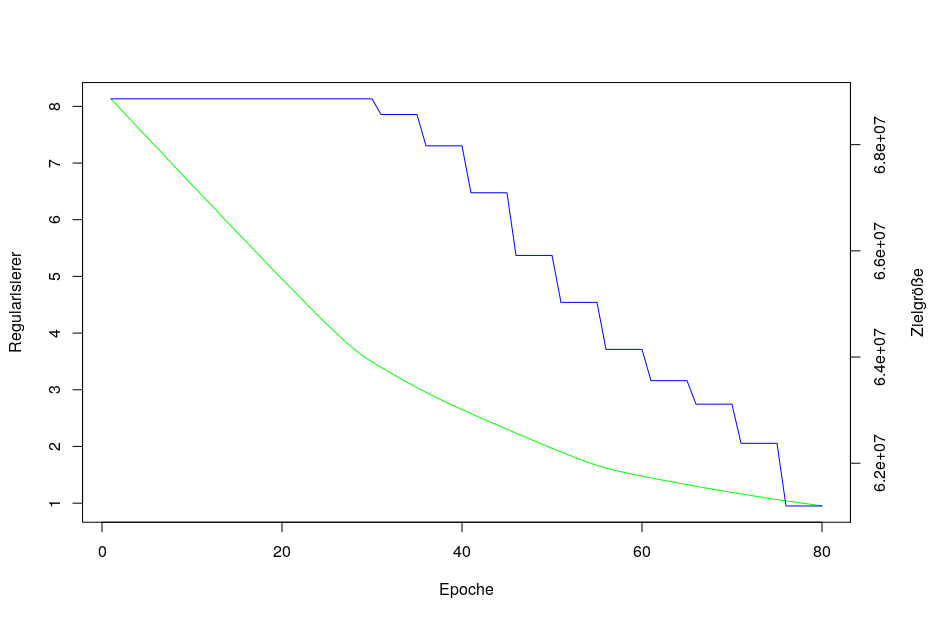
\includegraphics[width=0.47\textwidth]{KapitelPartB/Images/morph1.png}\label{abb:morphSize}}
     \hfill
     \subfloat[][]{
     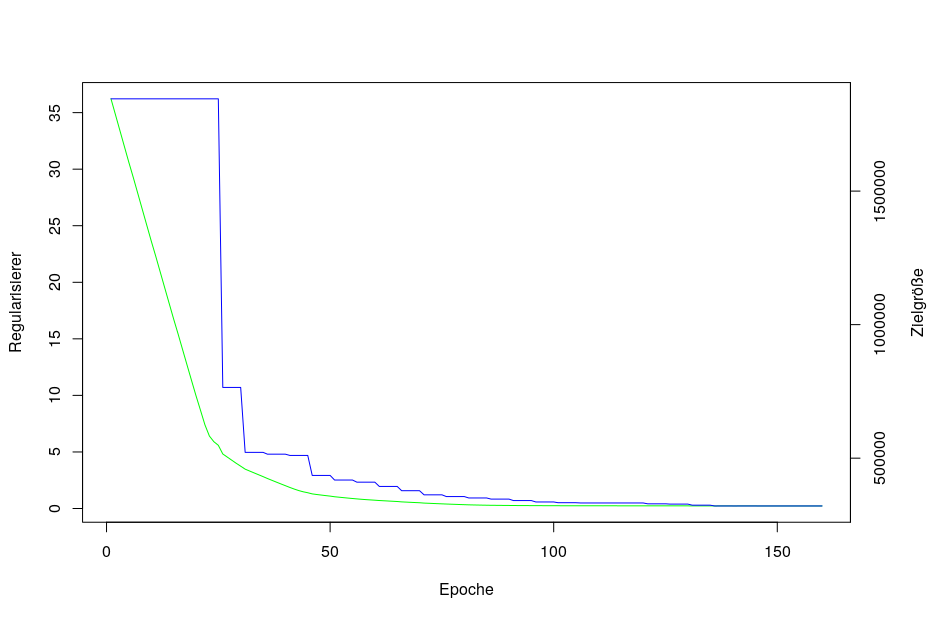
\includegraphics[width=.47\linewidth]{KapitelPartB/Images/morph2.png}\label{abb:morphFLOPs}
     }
     \caption{Vergleich Zielgröße mit Wert des Regularisierers für (a) FLOPs (b) Modellgröße }
     \label{abb:morph1}
\end{figure}

Der Effekt von verschieden großen $\lambda$ wird im nächsten Schritt untersucht. Zu diesen Zweck wird ein Netzwerk mit verschiedenen Werten für $\lambda$ trainiert. Auch hier werden nur die ersten beiden Schritte des MorphNet-Algorithmus mehrfach hintereinander durchgeführt. In Abbildung \ref{abb:morphFlops1} ist zu sehen, wie sich der Morph-Net Algorithmus bei verschiedenen $\lambda$ für die Zielgröße FLOPs verhält. Dabei wird das Netz jeweils für fünf Epochen trainiert und anschliessend wird das Netz beschnitten. Abhängig von der Größe von $\lambda$ wird dem Regularisierer mehr oder weniger Gewicht gegeben. Dies sorgt für eine unterschiedlich große Verkleinerungsrate. In Abbildung \ref{abb:morphSize1} ist abgebildet wie sich die Netzverkleinerungsraten verändern, bei der Zielgröße Modellgröße.  

\begin{figure}
     \centering
     \subfloat[][]{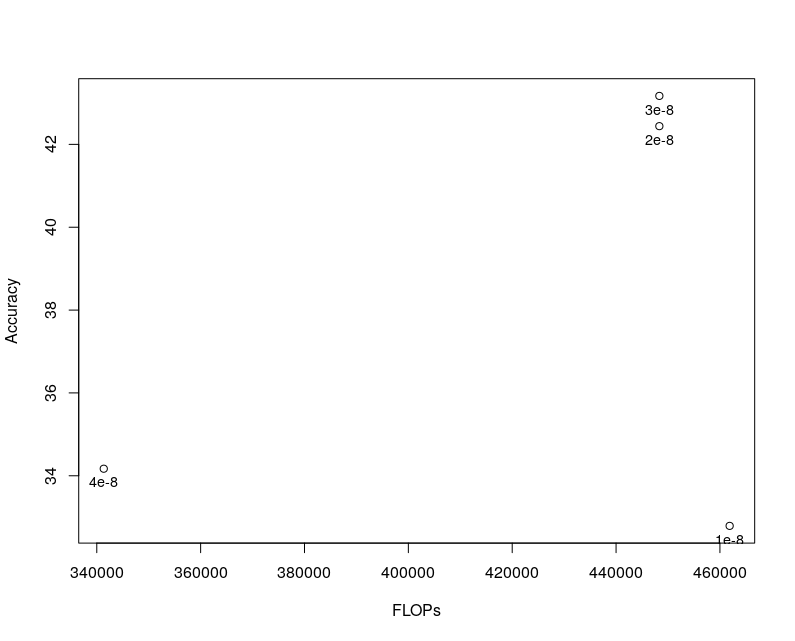
\includegraphics[width=0.47\textwidth]{KapitelPartB/Images/morph3.png}\label{abb:morphFlops1}}
     \hfill
%     \subfloat[][]{
%     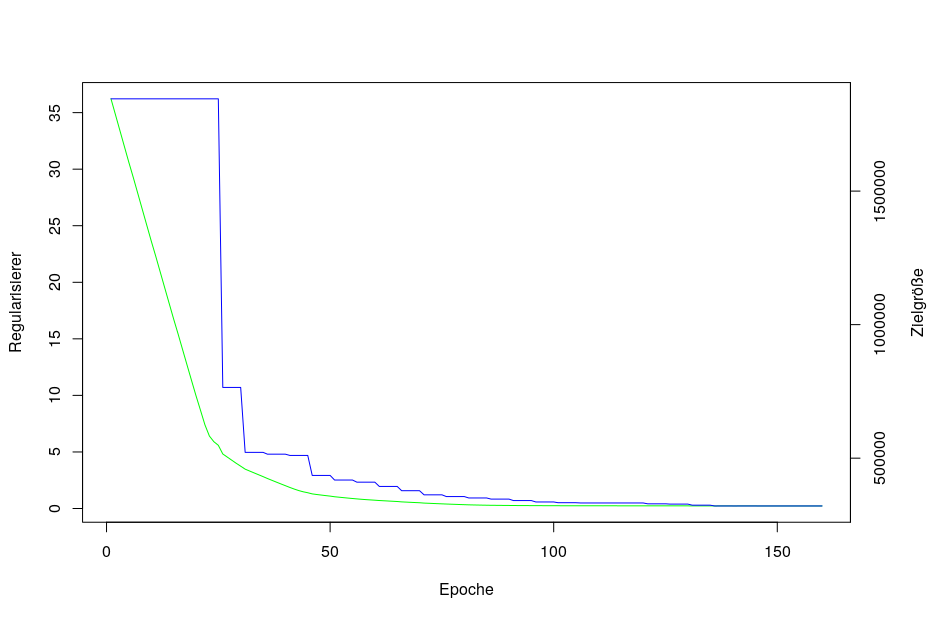
\includegraphics[width=.47\linewidth]{KapitelPartB/Images/morph2.png}\label{abb:morphSize1}
%     }
     \caption{Effekt verschieden großer $\lambda$ auf  (a) FLOPs (b) Modellgröße }
     \label{abb:morph2}
\end{figure}
Im letzten Schritt wird evaluiert, welchen Effekt die verschiedenen $\lambda$ auf den gesamten MorphNet-Algorithmus haben. Auf Grund dieser Ergebnisse werden die Parameter von MorphNet ermittelt, welches im nächsten Unterkapitel mit den Rahmenbedingungen von Kapitel \ref{sec:konzept} evaluiert wird.



\section{Evaluierung der Ergebnisse von MorphNet}

Die in Kapitel \ref{sec:konzept}  vorgestellte Vorgehensweise wir hier verwendet, um MorphNet zu evaluieren. Dies bildet die Grundlage zum Vergleich in Kapitel \ref{sec:vergleich}.











\chapter{Evaluation des Beschneidens des Netzes}\label{sec:ptexperimente}
\section{Evaluation bei gleichbleibender Batchgröße}

Die Untersuchung von PruneTrain basiert auf einer bereits vorgefertigten Implementierung \cite{ptImpl}. In dieser Implementierung ist alles bis auf die Anpassung der Batchgröße an das kleiner werdende Netz enthalten. Es wird das Ergebnis der Ausführung von PruneTrain auf der Hardware mit den Ergebnissen aus der Veröffentlichung verglichen \cite{prunetrain}. Ziel der Experimente ist es zu evaluieren, wie eine Änderung der verschiedenen Hyperparameter die Trainingszeit und die Accuracy beeinflusst. Im Gegensatz zur Veröffentlichung von PruneTrain wird hier statt auf mehreren GPUs nur auf einer GPU gerechnet. Bei der Evaluierung der Einflüsse werden die veränderbaren Hyperparameter von PruneTrain einzeln verändert, um den Einfluss der einzelnen Veränderungen zu untersuchen.  
Die veränderbaren Hyperparameter sind:
\begin{itemize}
 \item Lasso-Ratio $0,2$
 \item Rekonfigurationsinterval $5$
 \item Grenzwert $0,0001$
 \item Lernrate $0,1$
\end{itemize}
Hinter den veränderbaren Hyperparameter steht jeweils der Wert, den der Hyperparameter hat, wenn er im aktuellen Experiment nicht verändert wird, hat.
Betrachte eine feste Batchgröße von 256 über 180 Epochen und vergleiche diese mit dem Baseline-Netzes aus Kapitel \ref{sec:baseline}. 


\subsubsection{Einfluss von verschiedenen Lasso-Ratio Werten auf das Netz}
Die Lasso-Ratio gibt an, wie stark das Netz beschnitten werden soll. In diesen Experimenten wird die Lasso-Ratio von 0,05 bis 0,25 in 0,05er Schritten verändert. In Abbildung \ref{abb:lasso1} ist zusehen, dass mit steigender Lasso-Ratio durchschnittlich weniger Trainingszeit gebraucht wird. Für die durchschnittliche Trainingszeit einer Epoche wird das arithmetische Mittel über alle Epochen angewandt. Die Experimente werden dann nach ihrer Zugehörigkeit einsortiert und als Boxplot in Abbildung \ref{abb:lasso1} dargestellt. Trotz der nachlassenden Trainingszeit mit steigender Lasso-Ratio ist die Trainingszeit des Baseline-Netzes signifikant schneller. Dies ist durch den Overhead erklärbar, welcher durch das Beschneiden des Netzes entsteht.


In Abbildung \ref{abb:lasso2} ist die Accuracy der verschiedenen Experimente abgebildet. Es fällt auf, dass das Baseline-Netz im Mittel etwa schlechter ausfällt als die Experimente mit den Lasso-Ratio von 0,05 bis 0,15. Der Grund hierfür ist ein Overfitting. Das Overfitting wurde hier erkannt durch eine Trainingsaccuracy von 100,00 \% für mehrere Epochen ohne ein weiter steigende Validierungsaccuracy. 
\begin{figure}
     \centering
     \subfloat[][]{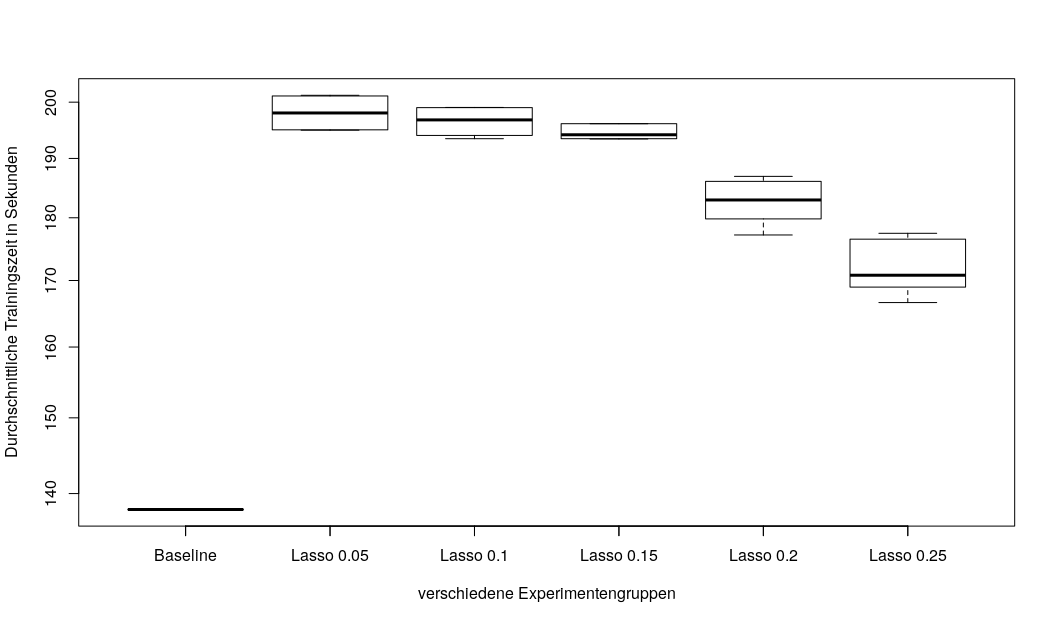
\includegraphics[width= .5\linewidth]{KapitelPartB/Images/lasso1.png}\label{abb:lasso1}}
     \hfill
     \subfloat[][]{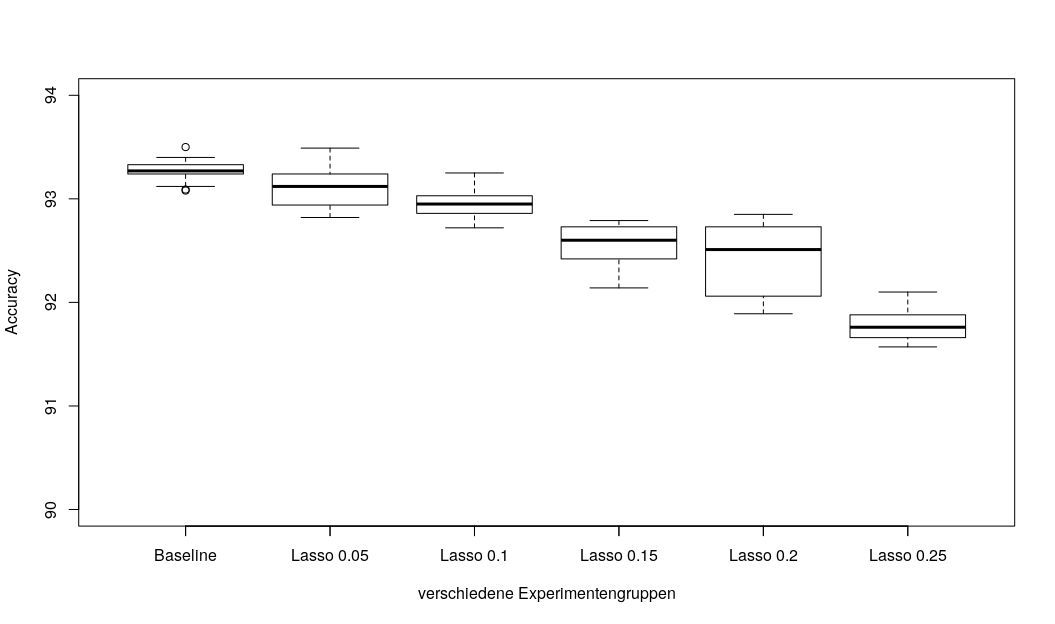
\includegraphics[width=.5\linewidth]{KapitelPartB/Images/lasso2.png}\label{abb:lasso2}}
     \caption{Lasso-Ratio Experiment: (a) Boxplot der durchschnittlichen Trainingszeit (b) Boxplot der Accuracys}
     \label{abb:lasso}
\end{figure}




\subsubsection{Experimente zum Rekonfigurationsintervall}
 Als nächste Größe wird der Einfluss des Rekonfigurationsintervalls überprüft. Die entsprechenden Grafiken sind in Abbildung \ref{abb:reconf} zu sehen. In Abbildung \ref{abb:reconf1} sind für die verschiedenen Experimente die Trainingszeiten pro Epoche zu sehen. Dabei werden drei verschiedene Rekonfigurationsintervalle (2,5 und 10) verglichen. In Abbildung \ref{abb:reconf1} lässt sich für die verschiedenen Trainingszeiten der Experimente zum Rekonfigurationsintervall kaum Unterschiede erkennen. Daher ist in Abbildung \ref{abb:reconf3} ein Boxplot ohne die Baseline Werte abgebildet. 
 
 
\begin{figure}
     \centering
     \subfloat[][]{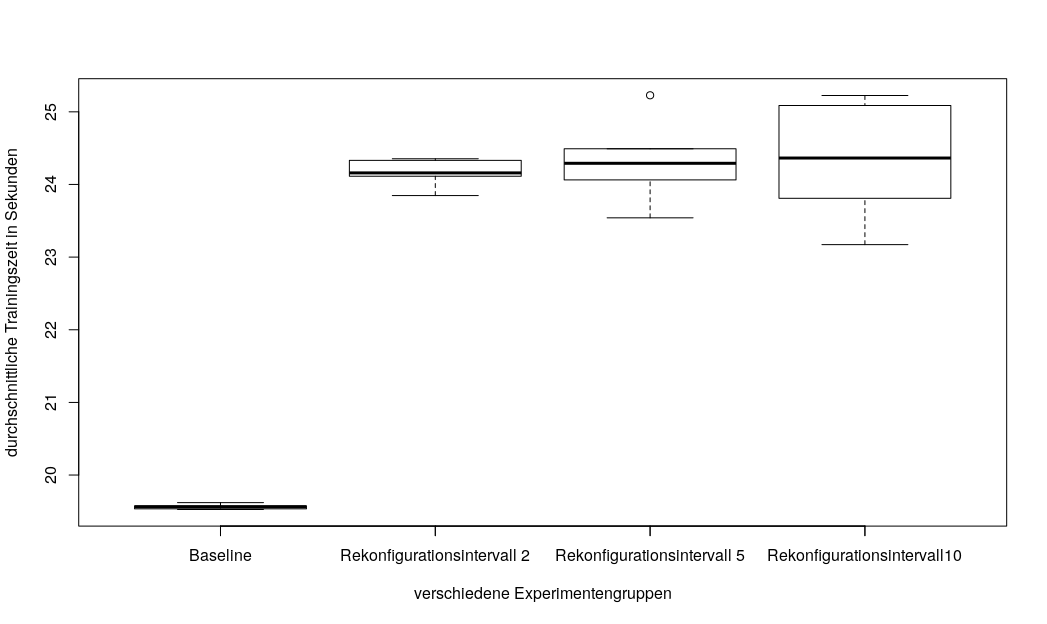
\includegraphics[width= .45\textwidth]{KapitelPartB/Images/reconf1.png}\label{abb:reconf1}}
     \hfill
     \subfloat[][]{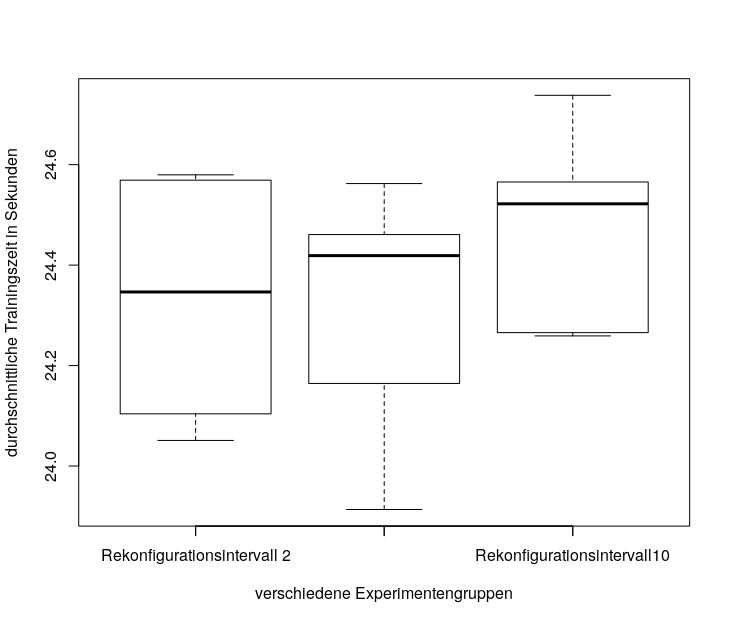
\includegraphics[width= .45\textwidth]{KapitelPartB/Images/reconf3.png}\label{abb:reconf3}}
     \\
     \subfloat[][]{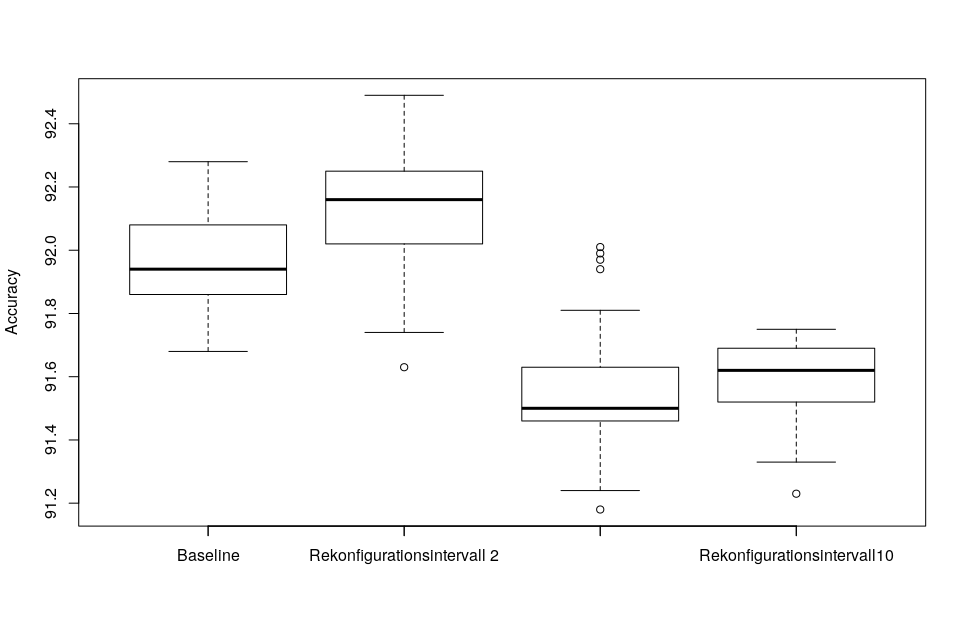
\includegraphics[width=.45\textwidth]{KapitelPartB/Images/reconf2.png}\label{abb:reconf2}}
     \caption{Experimente zum Rekonfigurationsintervall: (a) Boxplot der durchschnittlichen Trainingszeit (b) Boxplot der durchschnittlichen Trainingszeit ohne Baseline-Netz (c) Boxplot der Accuracys}
     \label{abb:reconf}
\end{figure}

 Mit Hilfe dieses Boxplots lässt sich erkennen, dass die durchschnittliche Trainingszeit aller Experimente mit dem Rekonfigurationsintervall steigt.
 
 In Abbildung \ref{abb:reconf2} ist zu sehen, wie sich die Accuracy bei diesen Experimenten verhält.
 \todo[inline]{Die Effekte in der Accuracy vom Baseline Netz zum Rekonfigurationsintervall sind wieder mit einem Overfitting zu erklären. Die Effekte vom Rekonfigurationsinterval 2 zu 5 und zu 10 sind auch mit Zunehmenden Overfitting je weniger geprunt wird zu erklären. Abhilfe mehr Experimente und zwar mit dem schmallen Baseline Netz}
 
\subsubsection{Experimente zur Lernrate}
Der Einfluss der Lernrate auf das Beschneiden des Netzes wird mit fünf verschiedenen Lernraten untersucht. Beginnend mit der Lernrate $0,2$ und für jede weitere der fünf Lernraten die Hälfte der vorherigen.
Die durchschnittliche Trainingszeit in Sekunden für verschiedene Lernrate ist in Abbildung \ref{abb:lr} zu sehen. Es ist deutlich zu sehen, dass mit sinkender Lernrate die Trainingszeit steigt. Das bedeutet, dass mit sinkender Lernrate weniger von Netz beschnitten wird.
 
 \begin{figure}
     \centering
     \subfloat[][]{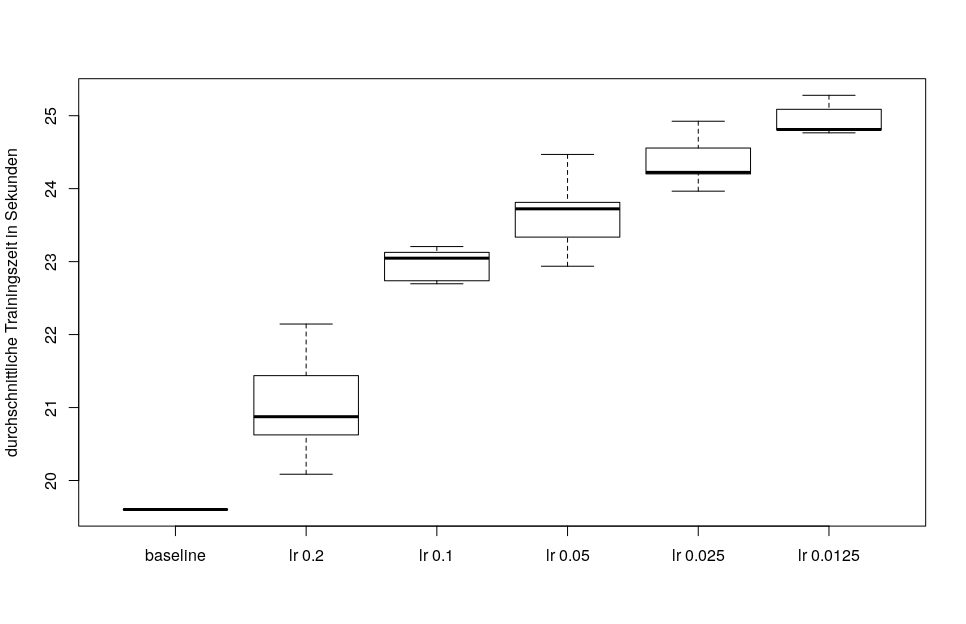
\includegraphics[width= .45\textwidth]{KapitelPartB/Images/lr1.png}\label{abb:lr1}}
     \hfill
     \subfloat[][]{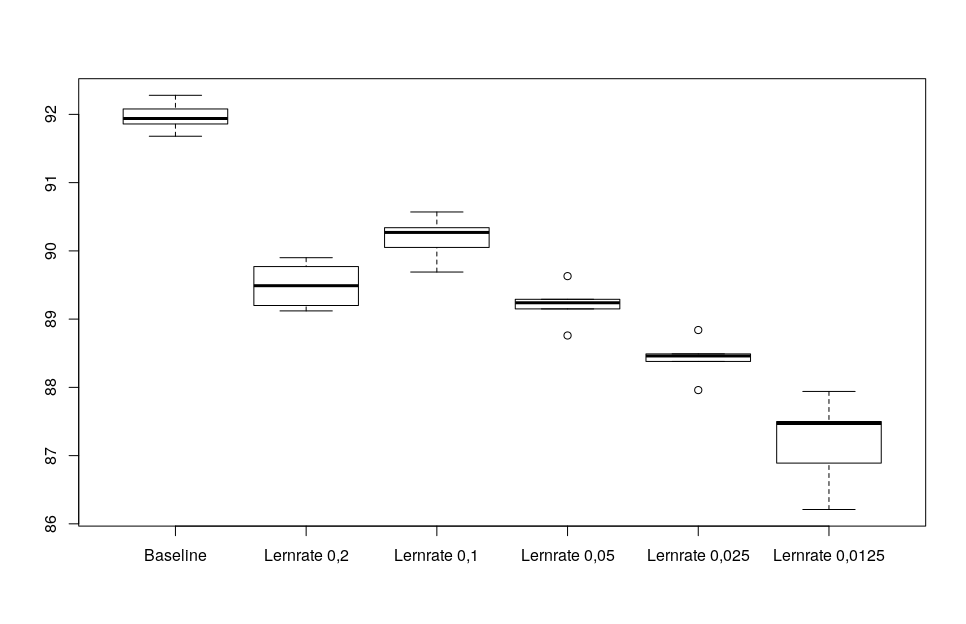
\includegraphics[width= .45\textwidth]{KapitelPartB/Images/lr2.png}\label{abb:lr2}}
     \caption{Experimente zuLernrate: (a) Boxplot der durchschnittlichen Trainingszeit (b) Boxplot der durchschnittlichen Trainingszeit ohne Baseline-Netz (c) Boxplot der Accuracys}
     \label{abb:lr}
\end{figure}

 In Abbildung \ref{abb:lr2} sind die Accuracy der verschiedenen Lernrate abgildet. Die Lernrate $0.1$ schneidet hier am Besten ab. Dies kann darauff zurück geführt werden, dass bei einer größeren Lernrate weniger Minima in der Verlustfunktion gefunden werden können. Der Effekt bei wesentlich kleineren Lernraten ist, dass der Trainingsprozess zwar mit jedem Schritt in die Richtung des Minimums geht, dabei aber durch die kleine Lernrate das tatsächliche Minimum innerhalb der 180 Epochen nicht erreicht.
 
 
 
 \subsubsection{Experimente zum Grenzwert}


\begin{figure}[h]
 \centering
 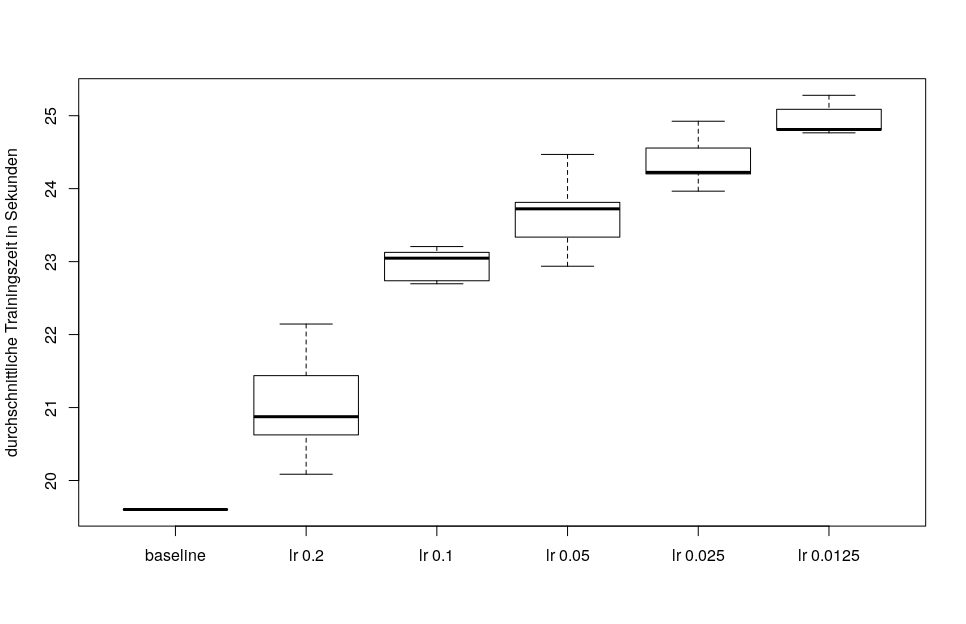
\includegraphics[width=0.8\textwidth]{KapitelPartB/Images/lr1.png}
 % lr1.png: 431x491 px, 96dpi, 11.41x12.99 cm, bb=0 0 323 368
 \label{ref:lra}
\end{figure}



 

\subsubsection{Diskussion der Methode}

Für die Evaluation des Beschneiden des Netzes werden in der Original-Veröffentlichung mehrere GPUs verwendet \cite{prunetrain}. Dies führt dazu, dass bereits in diesem Teil der Implementierung Trainingszeit durch verminderte Kommunikation zwischen den GPUs gespart wird. Da hier nur mit einer GPU evaluiert wird ergibt sich hier noch keine direkte Einsparung an Trainingszeit. Eine weitere Möglichkeit Trainingszeit zu sparen ergibt sich durch Erhöhen der Batchgröße bei kleiner werdendem Netz. Zu beachten ist hier, dass die Speicherauslastung gleich bleiben sollte und eine Vergleichbarkeit mit der Veröffentlichung zu gewährleisten. Diese Evaluierung wird in Kapitel \ref{sec:ptnew} durchgeführt.


\section{Experimente zur Anpassung der Batchgröße beim Beschneiden des Netzes}\label{sec:ptnew}

Die Anpassung der Batchgröße des Netzwerks in der Veröffentlichung arbeitet mit einer Grenze bis zu dieser der Speicher ausgelastet werden darf. 

Die Berechnung der maximalen Batchgröße für eine gegegebene Speichergrösse und Netzarchitektur wird in Kapitel \ref{sec:batch} beschrieben.

\subsection{Berchnung der Batchgröße abhängig vom Speicherverbrauch}\label{sec:batch}
Da sich in Pytorch der freie Speicher nicht direkt auslesen lässt wird mit Hilfe von Experimenten, die auf der GPU durchgeführt werden gemessen wie sich die Speicherauslastung verhält. In Abbildung \ref{abb:memory1} ist zu sehen, wie sich die Speicherauslastung proportional zur Batchgröße verhält. Es ist gut zu erkennen, dass der Zusammenhang linear ist. Die Passgenauigkeit dieses Zusammenhangs kann mittels einer linearen Regression bestimmt werden.  Daher wird  die rote Gerade wurde einer linearen Regression berechnet. Der maximale Abstand der gemessenen Punkte zur Gerade ist $0,19$ für Punkte, die unter der Gerade liegen sowie $0,67$ für Punkte die über der Gerade liegen. Zusammen mit der graphischen Übereinstimmung ergibt sich klar ein linearer Zusammenhang mit kleinen Abweichungen.
 \begin{figure}
     \centering
     \subfloat[][]{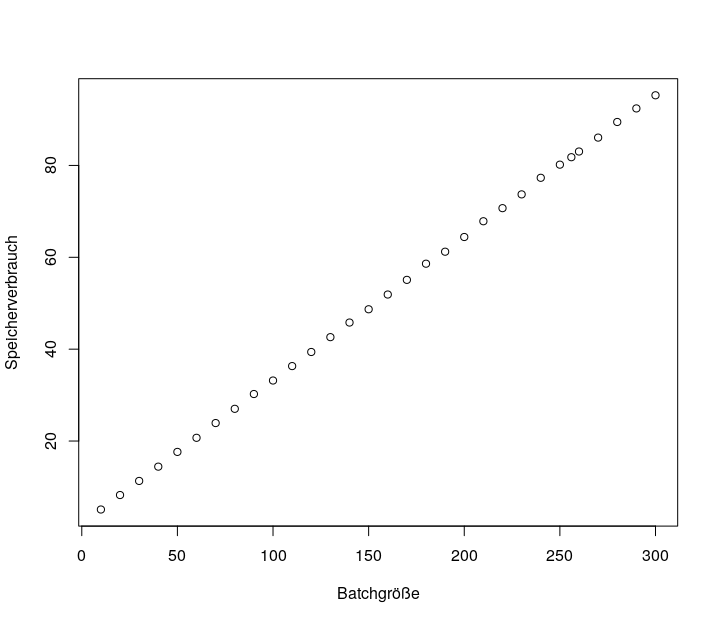
\includegraphics[width= .47\textwidth]{KapitelPartB/Images/memory1.png}\label{abb:memory1}}
     \hfill
     \subfloat[][]{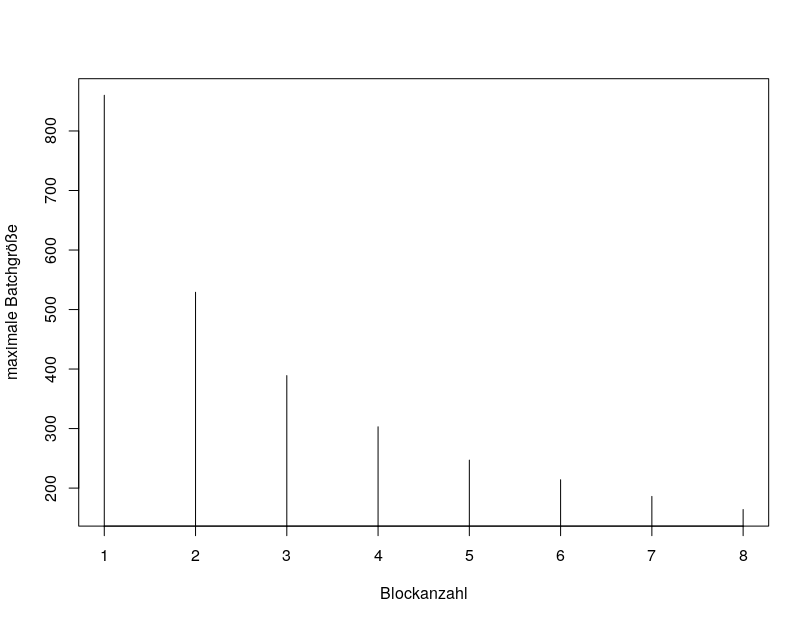
\includegraphics[width= .47\textwidth]{KapitelPartB/Images/memory2.png}\label{abb:memory2}}\\
     \subfloat[][]{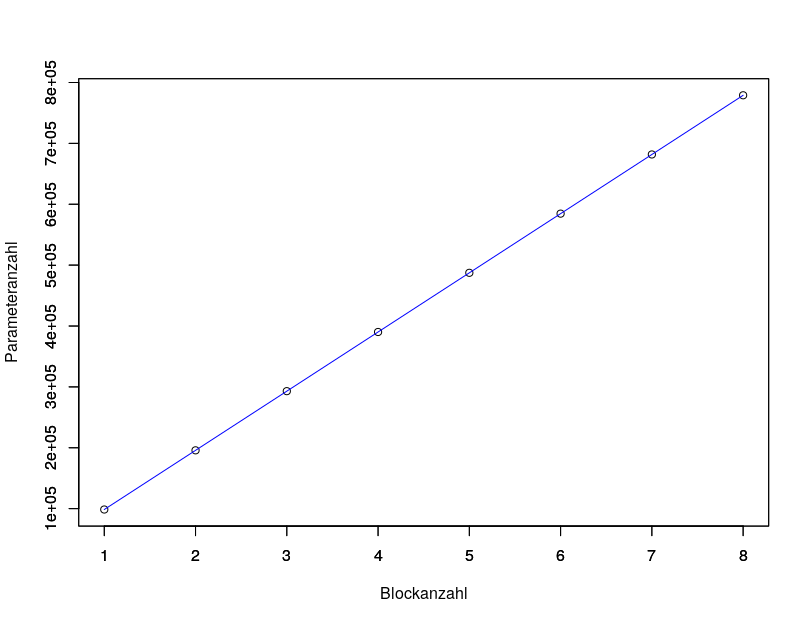
\includegraphics[width= .47\textwidth]{KapitelPartB/Images/memory3.png}\label{abb:memory3}}
     \hfill
     \subfloat[][]{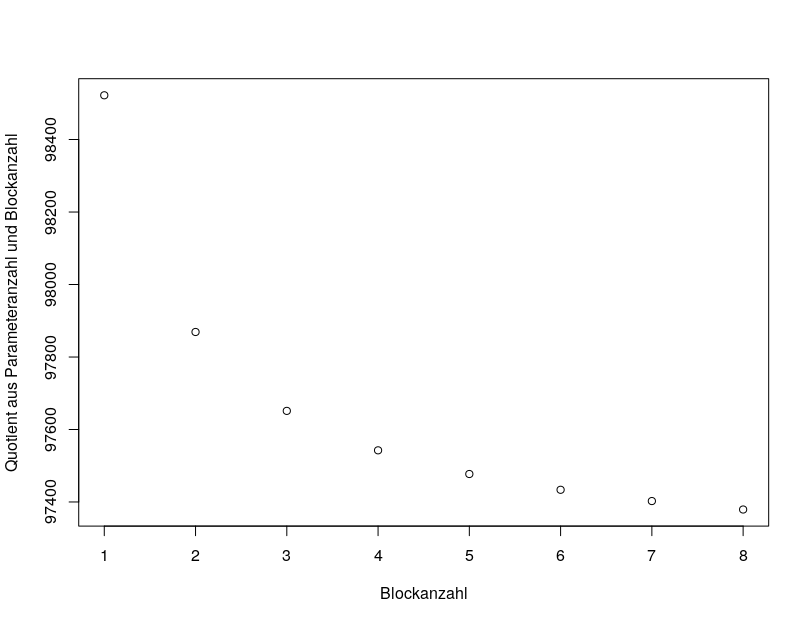
\includegraphics[width= .47\textwidth]{KapitelPartB/Images/memory4.png}\label{abb:memory4}}\\
     \subfloat[][]{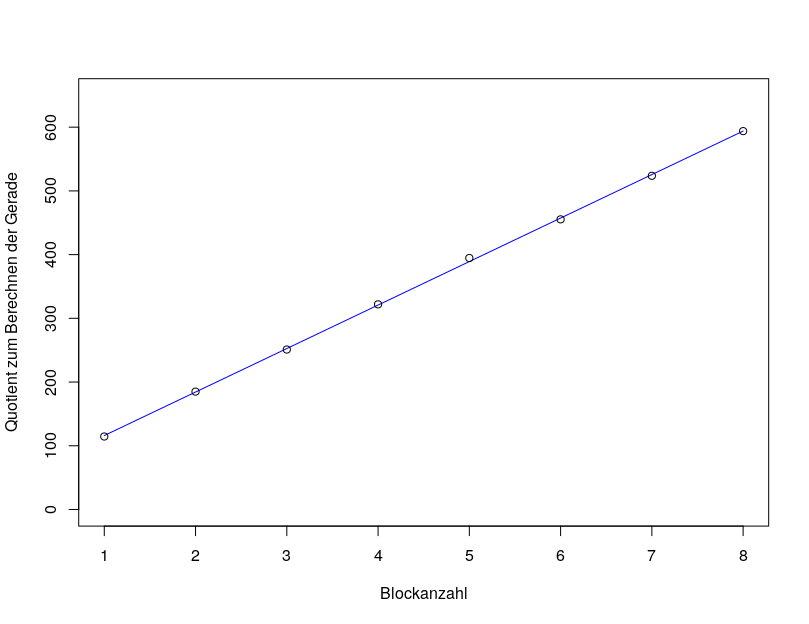
\includegraphics[width= .47\textwidth]{KapitelPartB/Images/memory5.png}\label{abb:memory5}}\\
          
     \caption{Darstellung des Berechnen der Geraden}
     \label{abb:memory}
\end{figure}
Durch diesen linearen Zusammenhang reicht es ein Modell zu bilden, welches für einen Wert des Speicherverbrauchs abhängig von der Netzarchitektur berechnet, wie groß die Batchgröße maximal sein darf. Zu diesem Zweck wird ein Netz mit drei Phasen betrachtet und ein Modell entwickelt mit dem sich die maximale Batchgröße berechnen lässt. Die maximale Batchgröße hängt ab von:

\begin{itemize}
 \item der Blockanzahl
 \item der Phasenanzahl und
 \item der Anzahl an Schichten pro Block
 \item Breite der Schichten je Phase
\end{itemize}
In Abbildung \ref{abb:memory2} ist abgebildet, wie sich die Blockanzahl bei gleichbleibender Speicherauslastung auf die maximale Batchgröße auswirkt. Die Blockanzahl wirkt sich wie zu sehen ist nicht linear auf die maximale Batchgröße aus. Betrachtet man hingegen den Zusammenhang zwischen Blockanzahl und Parameteranzahl, wie in Abbildung \ref{abb:memory3} abgebildet, so ergibt sich hier ein linearer Zusammenhang. In Abbildung \ref{abb:memory4} ist der Zusammenhang zwischen Blockanzahl und dem Quotienten aus Parameteranzahl und Blockanzahl zu sehen. Der Verlauf dieser Kurve ähnelt dem Verlauf von Abbildung \ref{abb:memory2}. In Abbildung \ref{abb:memory5} wird daher der Quotient aus diesen beiden Größen gegen die Blockanzahl geplottet und eine Gerade mit linearer Regression berechnet.
Um die Wahrscheinlichkeit zu prüfen, mit fälschlicherweise angenommen wird, dass in Abbildung \ref{abb:memory} ein linearer Zusammenhang besteht wird ein t-Test ausgeführt.
Es ergibt sich die Alternativ- und Nullhypothese:
\begin{align*}
 H_0: \text{Es besteht kein linearer Zusammenhang zwischen dem Quotienten } G \\
 \text{und der Anzahl von Blöcken} \\
 H_1: \text{Es besteht ein linearer Zusammenhang zwischen dem Quotienten } G \\ 
 \text{ und der Anzahl von Blöcken}
\end{align*}
Mit einem Signifikanzniveau von $\alpha =0,05$ und einem $p$-Wert von $p=3,824 \cdot 10^{-12}$ ist die Nullhypothese abzulehnen, und die Alternativhypothese anzunehmen. 

Mit Hilfe dieses linearen Zusammenhangs lässt sich bei gegebener Parameteranzahl $(PA)$ und Blockanzahl $(BA)$ die maximale Batchgröße $(BG)$ berechnen:

\begin{equation}
 BG=\frac{PA}{BA\left( 68,25 \cdot BA + 47,85\right)}
\end{equation}


Da einzelne Punkte einen maximalen Abstand von $d_{-}=2,07$ zur Geraden wurde das Ergebnis durch Multiplikation mit $0,98$ ein Sicherheitsabstand eingeführt.


\subsection{Evaluierung der Anpassung der Batchgröße an die Netzgröße}

Da sich für ein gegebenes Netz die Speicherauslastung abhängig von der Batchgröße ein linearer Zusammenhang ergibt, kann die Batchgröße direkt angepasst werden, sobald das beschnittene Netz für eine Epoche trainiert hat. Es wird per Dreisatz berechnet wie groß die Batchgröße sein darf, bei gegebener maximaler Speicherauslastung. In Abbildung \ref{abb:bSize1} ist zu sehen wie sich die durchschnittliche Trainingszeit pro Epoche entwickelt, bei Anpassung der Batchgröße. Für Abbildung \ref{abb:bSize1} werden zwei verschieden große Lasso-Ratio Werte $(LaR)$ $(0,2 \text{und} 0,25)$ getestet. Bei der Lasso-Ratio von $LaR=0,25$ ergibt sich ein Gewinn an durchschnittlicher Trainingszeit pro Epoche. 


 \begin{figure}
     \centering
     \subfloat[][]{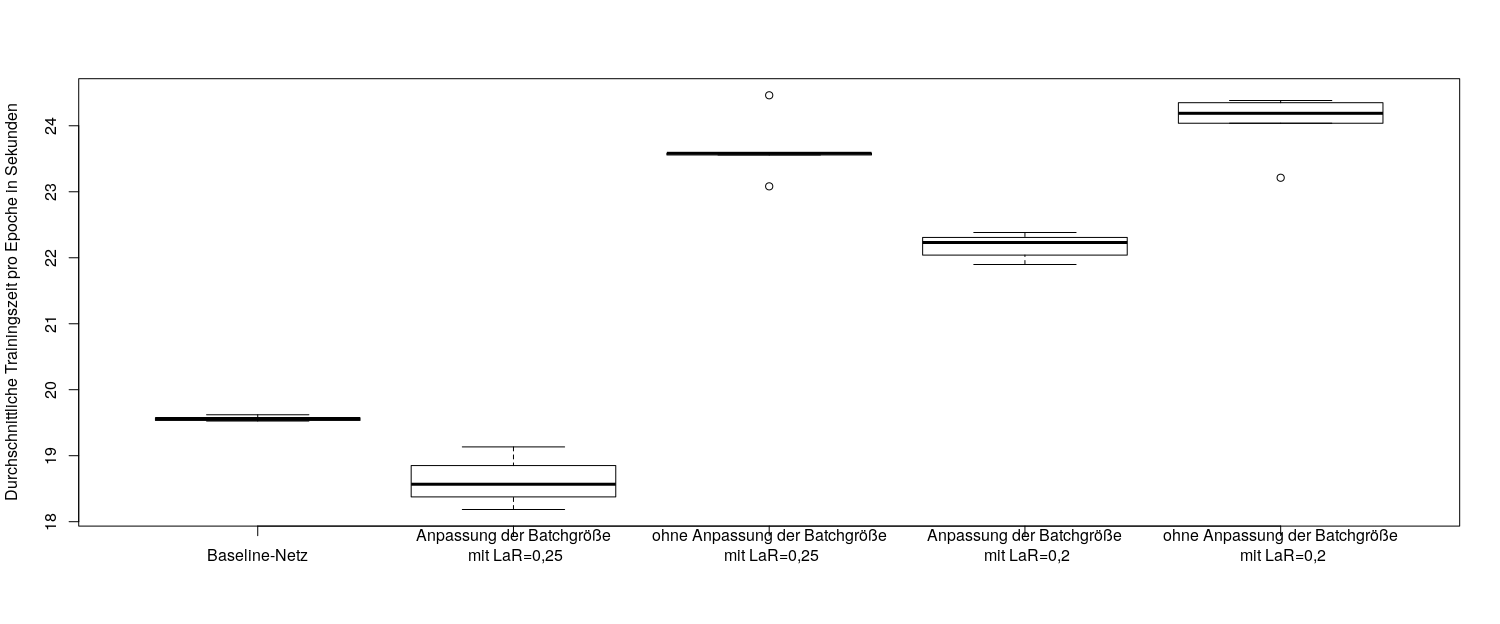
\includegraphics[width= .75\textwidth]{KapitelPartB/Images/bSize1.png}\label{abb:bSize1}}
     \hfill
     \subfloat[][]{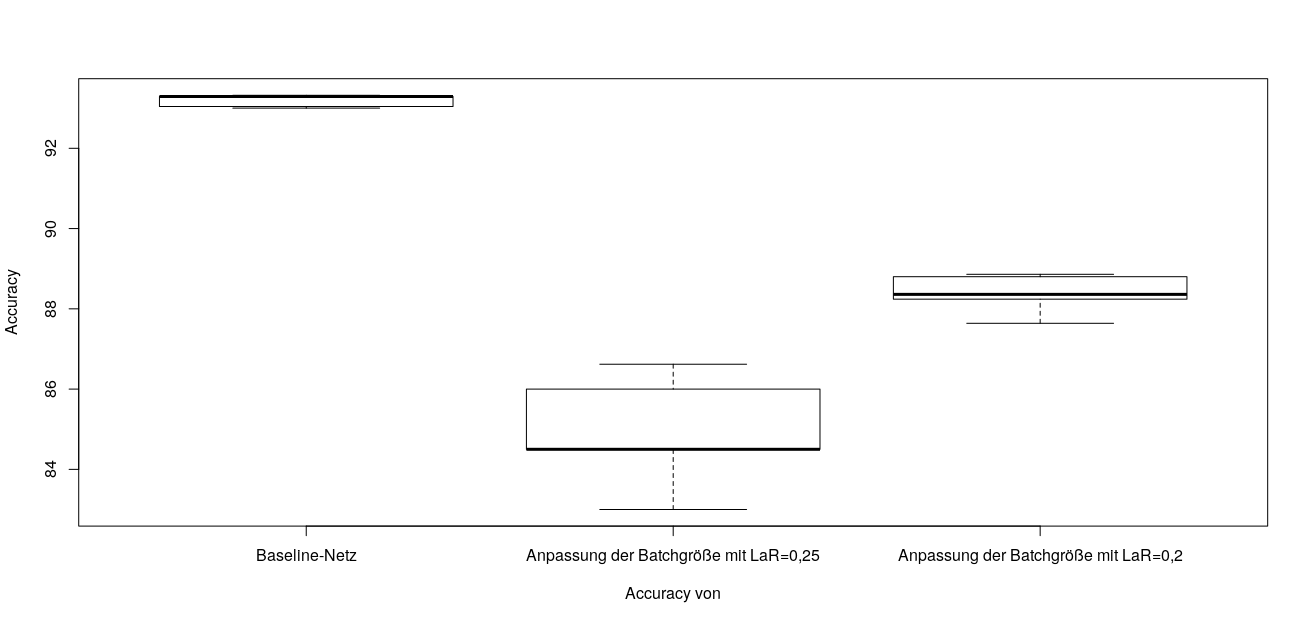
\includegraphics[width= .75\textwidth]{KapitelPartB/Images/bSize2.png}\label{abb:bSize2}}\\
     \caption{Vergleich von (a) Durchschnittlicher Trainingszeit (b) Accuracys von PruneTrain mit Anpassung der Batchgrößeund Baseline-Netz}
     \label{abb:bSize}
\end{figure}

In Abbildung \ref{abb:bSize2} ist zu sehen, wie gross der Accuracy-Verlust für das PruneTrain-Netz mit Anpassung der Batchgröße. Für PruneTrain mit einer Lasso-Ratio von 0,2 ergibt sich ein Accuracy Verlust von durchschnittlic xx,xx \%. Für eine höhere Lasso-Ratio ergibt sich ein Accuracy-Verlust von xx,xx \%.







\chapter{Evaluierung von Net2Net}\label{sec:net2netexperimente}
Die Operatoren zur Beschleunigung des Lernens durch Wissenstransfer werden in diesem Unterkapiel evaluiert. Diese Evaluierung arbeitet mit einer selbst erstellten Implementierung auf Grundlage der Veröffentlichung zum Thema Net2Net \cite{net2net}.

Die Evaluierung umfasst drei unterschiedliche Situationen, diese Situation sind analog zu den in der dazugehörigen Quelle \cite{net2net}. Die Evaluierung arbeitet mit einem ResNet, wie in Kapitel \ref{sec:baseline}.

In der ersten Situation wird der Operator für ein breiteres Netz verwendet, um ein schmalleres ResNet32 zu trainieren. 
In der zweiten Situation wird der Operator für ein tieferes Netz benutzt um zusätzliche Blöcke hinzuzufügen oder bestehenden Blöcken Schichten hinzuzufügen. In der dritten Situation werden beide Operatoren kombiniert. Mit der Kombination wird der Raum erkundet, ausgehend von einem Modell.
Die drei Situationen werden in den drei folgenden Unterkapiteln näher beschrieben. Anpassungen, wie eine Veränderung der Lernrate werden hier nicht vorgenommen.

\section{Evaluierung des Operators für ein breiteres Netz}
Evaluiert wird der Operator durch verschiedene Optionen, welcher Bereich des Netzes breiter gemacht wird:
\begin{itemize}
 \item Alle Phasen
 \item Eine ganze Phase
\end{itemize}
Wie in Kapitel \ref{sec:net2net} beschrieben werden beim Operator für ein breiteres Netz die Gewichte für die neu hinzugefügten Gewichte aus den ursprünglichen Gewichten ausgewählt und transformiert. Um zu evaluieren wie gut diese Methode funktioniert wird sie verglichen mit dem schmallen und breiten Baseline-Netz. Um die Methode der Initialisierung der zusätzlichen Kanäle zu evaluieren wird als Vergleich ein Netz trainiert, bei welchem die zusätzlichen zusätzlichen Gewichte zufällig initialisiert werden.
\color{blue1}
Zum Anwenden des Operators für ein breiteres Netz muss entschieden werden, in welcher Epoche und um welchem Faktor das Netz breiter gemacht werden soll. Wie in Kapitel \ref{sec:baseline} erörte schneidet das Netz besser ab, wenn die Lernrate während dem Training mehrfach angepasst wird. Das heisst, bei einem nicht zufriedenstellenden Ergebnis gibt es hier zwei Möglichkeiten, wie weiter verfahren werden soll.

In Abbildung \ref{abb:deeper1} ist der Verlauf der Trainingsaccuracy des schmallen Baseline Netzes über 180 Epochen ohne Anpassung der Lernrate zu sehen. Dabei ist zu sehen, dass das Netz nicht konvergiert. Zunächst wird der Zeitpunkt gesucht, ab dem das Netz nicht mehr besser wird im Durchschnitt. Damit die Entscheidung in einer Epoche stärker von den näher liegenden vergangenen Epochen abhängig ist, wird ein exponentiell gewichteter Mittelwert berechnet. In die Berchnung eingehen werden letzten $n$ Werte, für ein festes $n$.
Abbildung \ref{abb:deeper2} zeigt den Verlauf dieses Mittelwert für $n=10$ (Blau) und $n=30$ (Grün).
\begin{figure}
     \centering
     \subfloat[][]{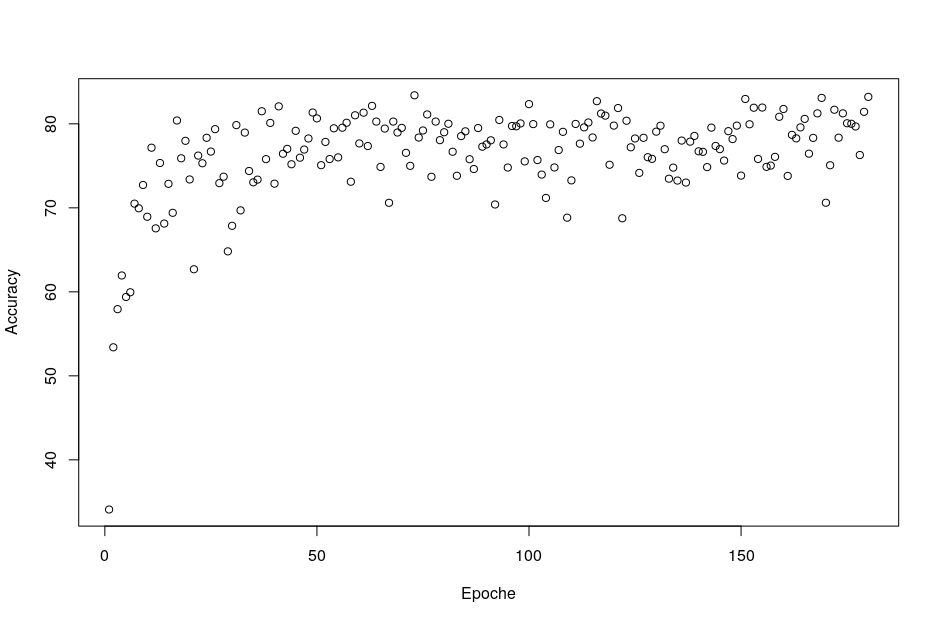
\includegraphics[width= .47\textwidth]{KapitelPartB/Images/deeperD1.png}\label{abb:deeper2}}
     \hfill
     \subfloat[][]{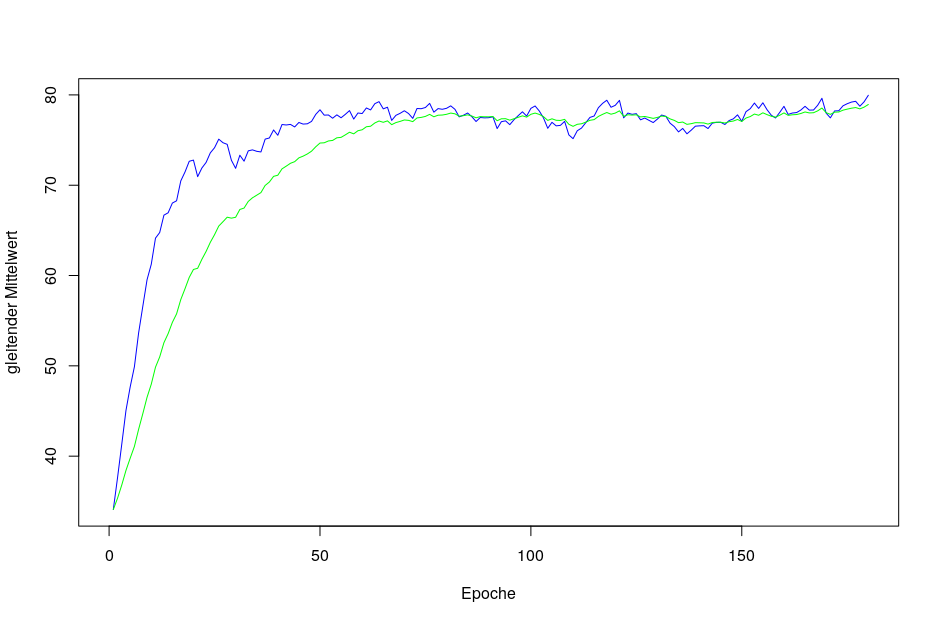
\includegraphics[width= .47\textwidth]{KapitelPartB/Images/deeperD2.png}\label{abb:deeper2}}\\
     \caption{}
     \label{abb:memory}
\end{figure}
Im nächsten Schritt muss anhand eines Entscheidungskriteriums 


\color{black}
\subsection{Verbreitern aller Phasen}
Mit Hilfe verschiedener Trainingsprotokolle wird untersucht, wie der Operator für ein breiteres Netz die Klassifikationsleistung des Netzes verändert.
Zunächst wird überprüft, welches Ergebnis bei Anwendung des Operators für ein breiteres Netz auf das schmalle Baseline-Netz nach 180 Epochen Training herauskommt. Nachdem Anwenden des Operators wird mit dem gleichen Trainingsprotokoll für weitere 180 Epochen trainiert. In Abbildung \ref{abb:allN2N1} ist abgebildet, wie der Verlauf der Accuracy für Net2Net mit zwei verschiedenen Möglichkeiten, die neuen Gewichte zu initialisieren, ist. In Blau dargstellt wird der Verlauf der Accuracy für die zufällige Initialisierung der neuen Gewichte durch das Verbreitern des Netzes.
Es ergibt sich, wie in der größeren Abbildung \ref{abb:allN2N2} zu sehen ist eine minimale Verschlechterung durch das Anwenden des Operator für ein breiteres Netz im Vergleich zum Baseline-Netz.
 \begin{figure}
     \centering
     \subfloat[][]{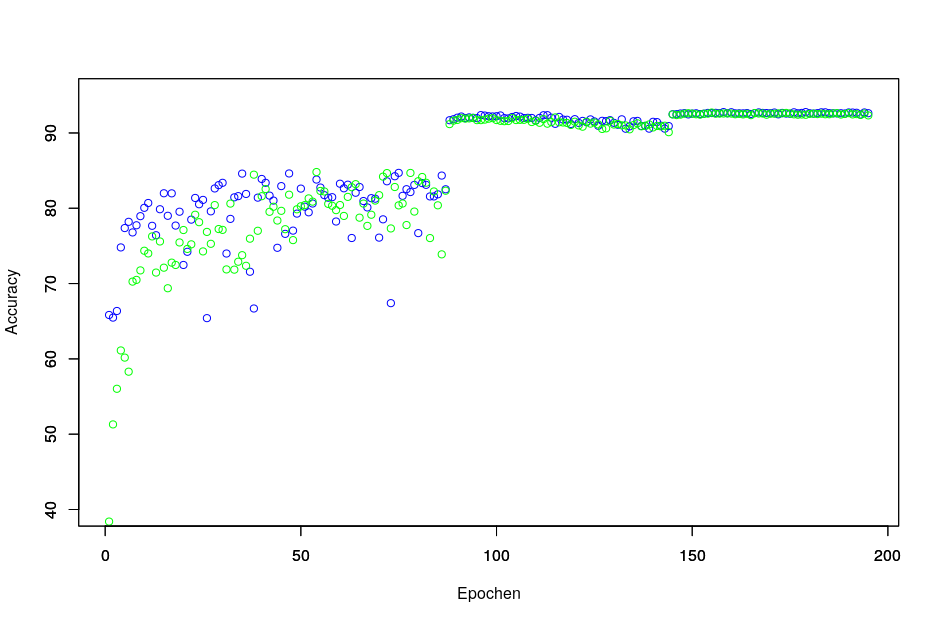
\includegraphics[width= .47\textwidth]{KapitelPartB/Images/n2nWiderAll1.png}\label{abb:allN2N1}}
     \hfill
     \subfloat[][]{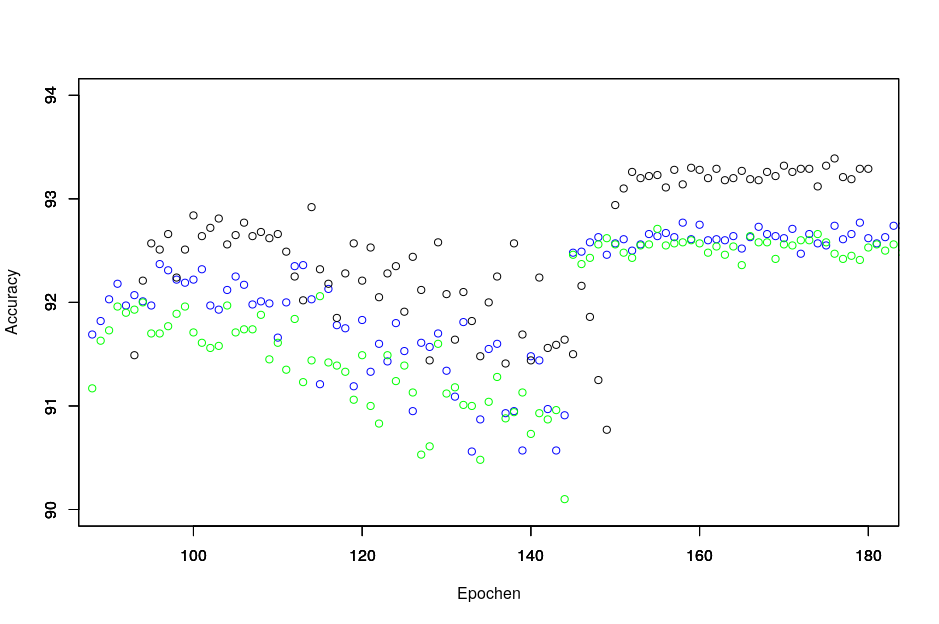
\includegraphics[width= .47\textwidth]{KapitelPartB/Images/n2nWiderAll2.png}\label{abb:allN2N2}}\\
     \caption{Vergleich der Accuracy bei verschiedenen Initialisierungsmöglichkeiten des Operators für ein breiteres mit dem Baseline Netz: (a) alle Epochen (b) Zoom auf die Epochen 90 bis 180. Blau zeigt die Accuracy der Initialisierung der zusätzlichen Gewichte mit zufälligen Werten. Grün zeigt die Initialisierung mit den Werten aus dem restlichen Tensor. Schwarz zeigt das Baseline-Netz als Vergleich.}
     \label{abb:memory}
\end{figure}
Um den Operator für ein breiteres Netz besser verwenden zu können wird im nächsten Schritt übrprüft, ob mit einer häufigeren schrittweisen Anpassung der Lernrate und mit weniger trainierten Epochen nach Anwenden des Operator ein besseres Ergebnis möglich ist.


\section{Evaluierung des Operators für ein tieferes Netz}
Zur Evaluierung des breiteren Netzes wird zunächst wie in der Veröffentlichung jeder Block um eine Schicht erweitert. Dabei werden die zusätzlichen Schichten wie in Kapitel \ref{sec:deep} beschrieben initialisiert. Als Vergleich dient das Baseline-Netz aus Kapitel \ref{sec:baseline}.

\todo{Ergebnisse}

Eine weitere Verwendung des Operators für ein tieferes Netz ist die Möglichkeit einen neuen Block hinzuzufügen. Nur ein einfaches Hinzufügen würde hier zu Problemen führen. Der Grund hierfür ist Abbildung \ref{abb:deeper} dargstellt. Dabei soll an einer Verbidung, die bisher die Daten von einer Schicht zur nächsten transportiert ein neuer Block inklusive Kurzschlussverbindung entstehen. Der hinzuzfügende Block blau \todo{blau markieren} markiert. Der neue Block soll wie die Kurzschlussverbindung die Identität berechnen. Betrachtet $x$ als Größe der Identität. Dann wird hier mit dem neuen Block staat $x$ das doppelte, also $``X$ berechnet. Um dieses Problem zu umgehen wird an jeder Additionsstelle für eine Kurzschlussverbindung eine Multiplikation mit 0,5 berechnet (rechte Seite der Grafik). So wird nicht mehr $x$ sondern $0,5x +0,5x=x$ berechnet.

Zunächst wird dieses Netz trainiert ohne einen Operator anzuwenden. In Abbildung \ref{abb:BaselineMul1} ist ein Boxplot abgebildet, der die Accuracy des Netzes mit zusätzlichen multiplikativen Faktoren mit dem Baseline-Netz vergleicht.

 \begin{figure}
     \centering
     \subfloat[][]{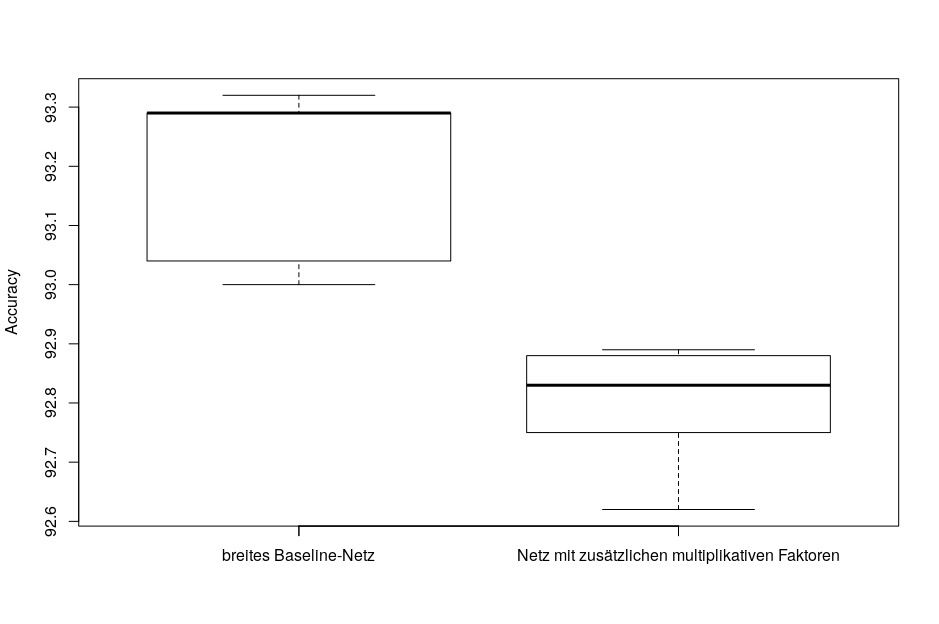
\includegraphics[width= .75\textwidth]{KapitelPartB/Images/baselineMul1.png}\label{abb:BaselineMul1}}
     \hfill
     \caption{Vergleich von }
     \label{abb:BaselineMul}
\end{figure}


\begin{figure}[h]
 \centering
 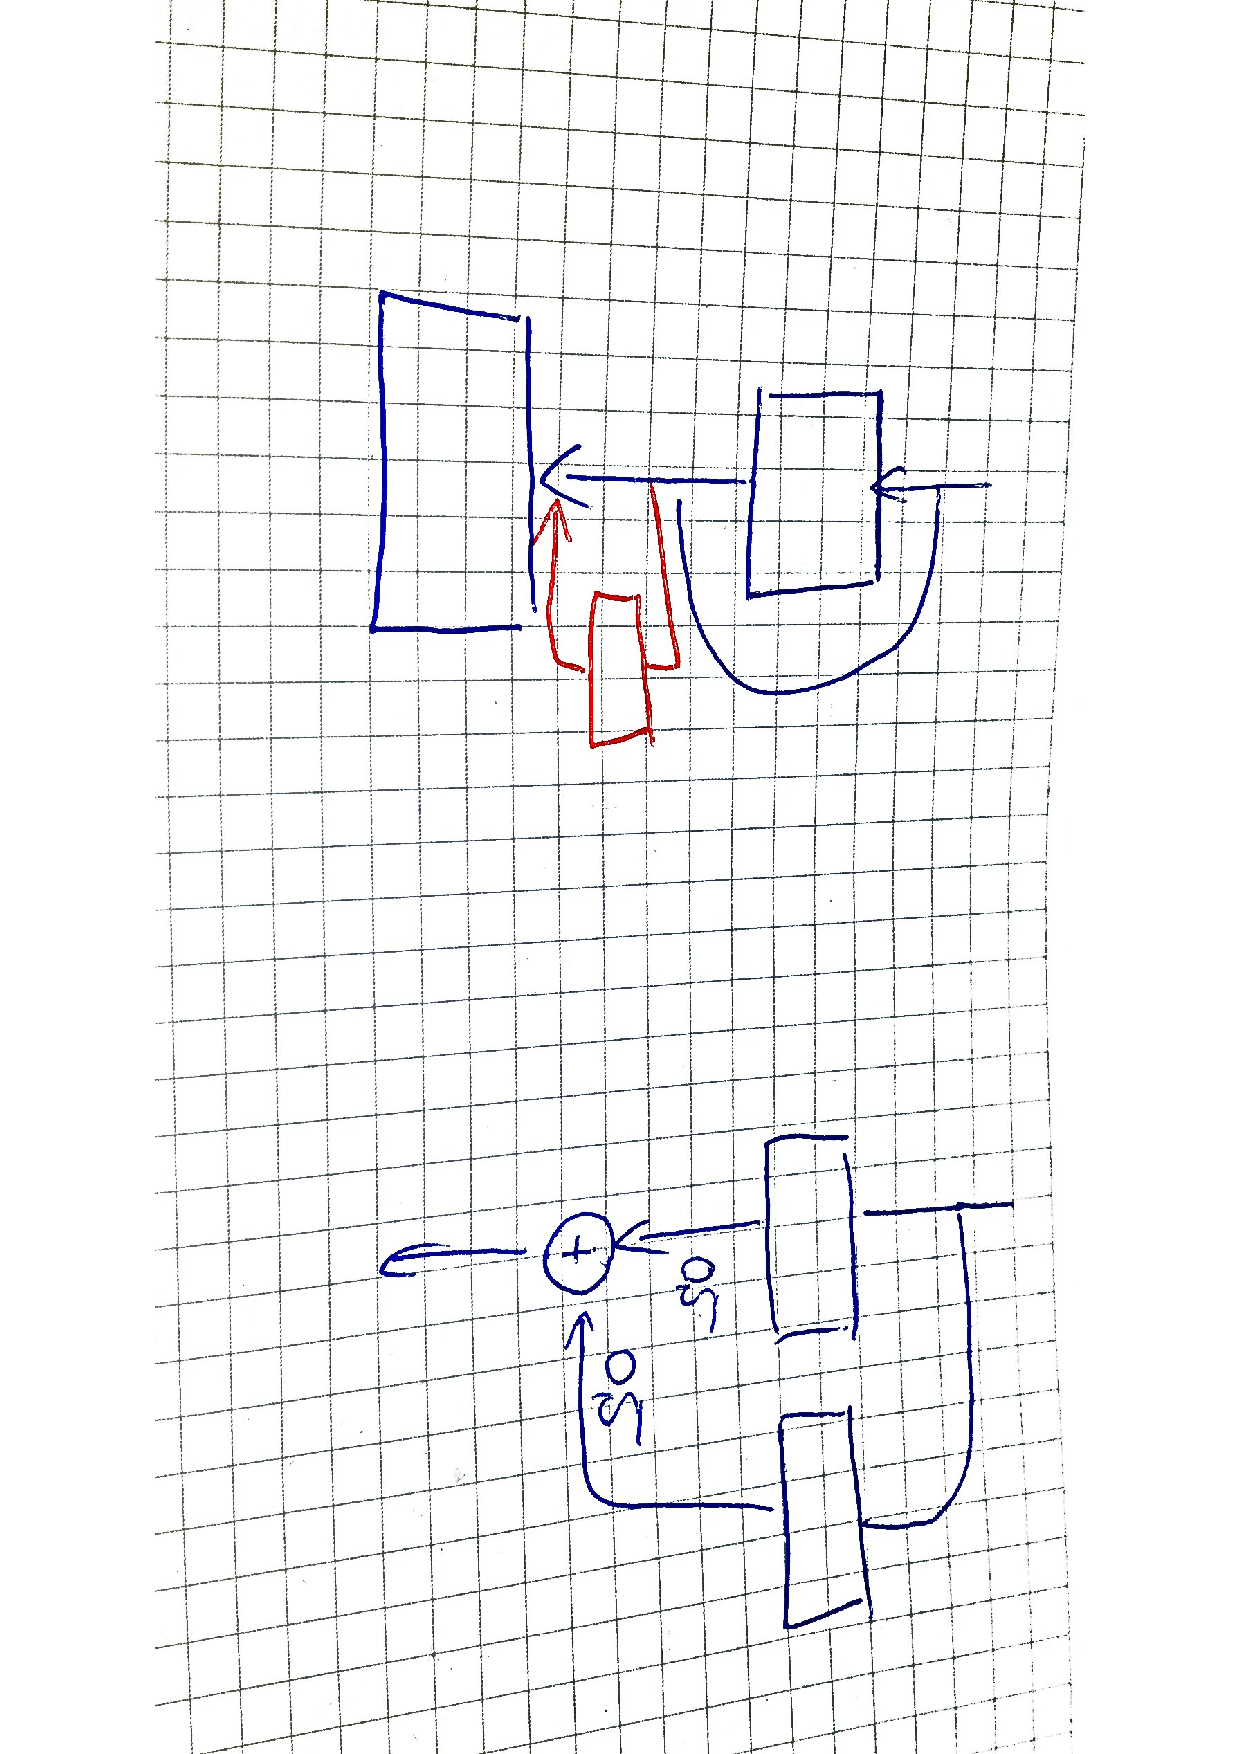
\includegraphics[width=0.5\textwidth, angle=90]{KapitelPartB/Images/deeper.pdf}
 % deeper.pdf: 0x0 px, 300dpi, 0.00x0.00 cm, bb=
 \label{abb:deeper}
\end{figure}




\section{Erkunden des Modellraums}

 \begin{figure}
     \centering
     \subfloat[][]{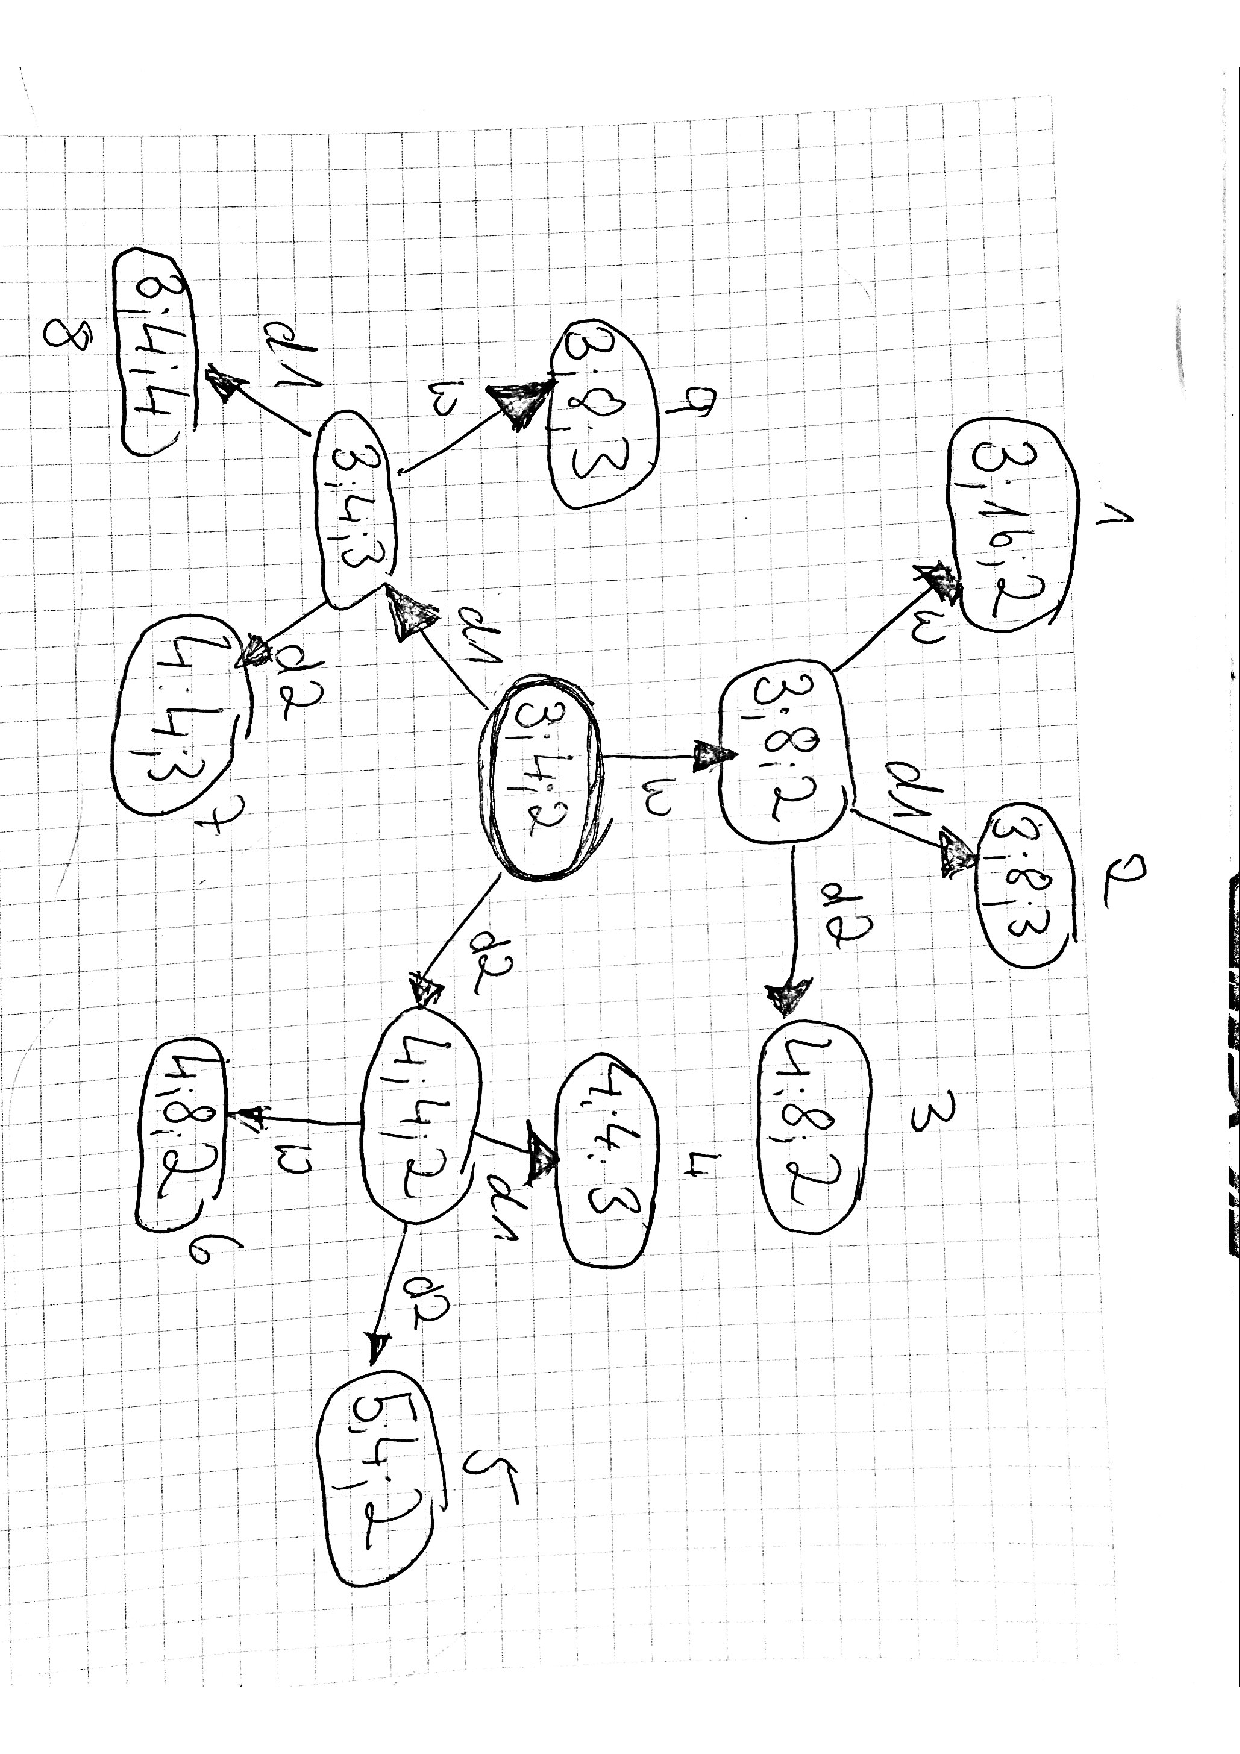
\includegraphics[width= .75\textwidth, angle=90]{KapitelPartB/Images/deeperRoom.pdf}
     \label{abb:deeperRoom1}}
     \caption{Anzahl an Blöcken pro Phase; Breite der ersten Schicht; Schichten pro Block}
     \hfill
\end{figure}


\chapter{Evaluierung der Kombination von PruneTrain und Net2Net }\label{sec:ptpnet2net}
Adaptive Kombination of prune and net2net

AKoPaN

Für die Kombination betrachten wir zunächst den Ausgang eines PruneTrain-Durchlaufs über 180 Epochen mit verschieden breiten Netzen:

4,8,16


8,16,32


16,32,64


und verschieden tiefen Netzen:

[3,3,3]


[4,4,4]




Gestartet wird wie bei Morphnet einmal mit 


4,8,16 und mit 


8,16,32
jeweils mit 3 Blöcken pro Phase
anlaog zu Kapitel 4.


um das Grösserwerden des Netzes nicht ausarten zu lassen sollte es nicht größer werden als 
das [5,5,5] er Netz mit 16,32,64 als maximalen Größe vorgegeben.




Drei Probleme können beim Training des Ntzes auftauchen:
\begin{itemize}
 \item Underfitting
 \item Overfitting
 \item Saturation
 \item Rumspringen ohne eine Tendenz zur Verbesserung
\end{itemize}

Underfitting erkennen wir durch einen immer noch recht hohen Trainingsfehler und relativ wenig Pruning.


Sowohl bei Hinzufügen von neuen Blöcken als auch beim Breiter machen des Netzes kann Overfitting passieren. Kommt es zu Overfitting ist es möglich, den Lasso-Ratio koeffizient weiter zu erhöhen, oder den Grenzwert zum Beschneiden des Netzes zu Erhöhen. Das heisst es ist nötig, Overfitting zu erkennen. Dies wird hier durch Abstand von Trainings und Validierungsfehler. Wird der Abstand hier grösser bei einer Zunnahme des Validierungsfehlers oder  ist die Testaccuracy bei 100 \% angekommen, wird Overfitting diagnostiziert.


Saturation
Bilde aus den letzten 10 Validierungsaccuracy jeweils ein exponentiel geglättetes Mittel gewichtetes Mittel. Zeigt dieses Mittel keine Verbesserung innerhalb der nächsten 10 Epochen -> early stop und je nach vorliegen von Under oder Overfitting weiterverfahren.



\chapter{Vergleich}\label{sec:vergleich}

\begin{comment}
\chapter{Additive Verfahren}

\subsection{Zahlenformate}\label{sec:zahlen}
\todo[inline]{Text fertig schreiben; etwa 4 Stunden}
\begin{itemize}
 \item FP16 bereits probiert
\end{itemize}


FP16 nur auf RTX 2080 sinnvoll
Bietet nach erster Messung etwa 28 \% Prozent Gewinn.

Code für dieses Verfahren liegt vor: Amp apex von Nvidia

AMP bietet 3 mögliche Optimierungsstufen:

O1
Patch all Torch functions and Tensor methods to cast their inputs according to a whitelist-blacklist model. Whitelist ops (for example, Tensor Core-friendly ops like GEMMs and convolutions) are performed in FP16. Blacklist ops that benefit from FP32 precision (for example, softmax) are performed in FP32. O1 also uses dynamic loss scaling, unless overridden.

02
casts the model weights to FP16, patches the models forward method to cast input data to FP16, keeps batchnorms in FP32, maintains FP32 master weights, updates the optimizer’s paramgroups so that the optimizer.step() acts directly on the FP32 weights (followed by FP32 master weight-FP16 model weight copies if necessary), and implements dynamic loss scaling (unless overridden). Unlike O1, O2 does not patch Torch functions or Tensor methods.


O3
may not achieve the stability of the true mixed precision options O1 and O2. However, it can be useful to establish a speed baseline for your model, against which the performance of O1 and O2 can be compared. If your model uses batch normalization, to establish speed of light you can try O3 with the additional property override keepBatchnormfp32=True (which enables cudnn batchnorm, as stated earlier).

Hier nur O0, O1 und O2 dargestellt, da O3 absolut nicht mithalten kann was Performance angeht.

\begin{figure}[h]
 \centering
 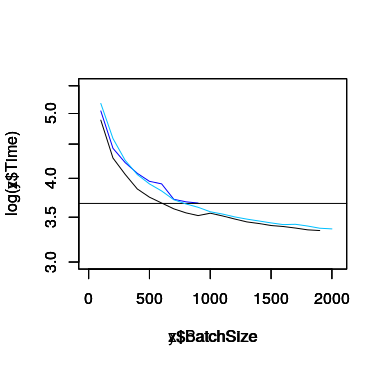
\includegraphics[width=0.8\textwidth]{KapitelPartB/Images/timeVsBatchSize_Amp.png}
 % timeVsBatchSize_Amp.png: 387x367 px, 96dpi, 10.24x9.71 cm, bb=0 0 290 275
 \caption{Vergleich Trainingszeit einer Epoche für verschiedene Optimierungsstufen von Amp Apex. DunkelBlau=O0; Schwarz = O1; Hellblau=O2}
 \label{fig:amp}
\end{figure}
\url{https://developer.download.nvidia.com/video/gputechconf/gtc/2019/presentation/s9998-automatic-mixed-precision-in-pytorch.pdf} zeigt, dass bezüglich der Accuracy kein Verlust zu erwarten ist.

Da O2 gegenüber O1 keinen signifikanten zusätzlichen Gewinn bringt nutze O1.



\subsection{LARS}\label{sec:lars}
\todo[inline]{Experimente fast fertig (3x mal auf einer Graka für 50 min); dann etwa 3 Stunden fürText + Evaluierung}




Es stellt sich die Frage, ob das einen so grossen Einfluss auf die Ausführungszeit hat.



Man sieht, dass mit steigender Batchgröße die Ausführungszeit sinkt. 

Errechne zusätzlich noch ein Modell, wo abhängig von der Modellgrösse währenddem Pruning die Batchgrösse angepasst wird.





\subsection{Beschleunigung der Berechnung des Gradientenabstiegverfahren}
\todo[inline]{ab hier löschen}

Accelerating CNN Training by Sparsifying Activation Gradients funktioniert nur auf Toy-Benchmarks 


\subsubsection{Weight Normalization: A Simple Reparameterization
to Accelerate Training of Deep Neural Networks}


Könnte funktionieren. Code für Lasagne: https://github.com/TimSalimans/weight\_norm


\subsubsection{Accelerating Deep Neural Network Training with Inconsistent Stochastic Gradient Descent}

Interessant bisher kein Code verfügbar

\subsubsection{Accelerated CNN Training Through Gradient Approximation }

Interessant bisher kein Code verfügbar


\end{comment}
